\chapter{\kadaib}
\section{\purpose}
この実験では,画像に対してフィルタの適用や色空間を変換する.\par
\paragraph{画像フィルタ} 画像に対して,フィルタを適用するとはどのようなことか?我々は,携帯電話の写真アプリケーションを用いて,写真を「加工」する.
我々は「加工」という行為を「フィルタをかける」と呼ぶが,この「フィルタ」という言葉と,画像処理におけるフィルタは意味が異なる.
画像処理におけるフィルタは,画像ないに含まれる雑音を除去したり,特徴を抽出したりすることで欠陥検出をより円滑に行うための基本処理を指す\cite{画像フィルタ}.
\newcommand{\originimg}{\texttt{original\_img}}
\newcommand{\wgnimg}{\texttt{wgn\_img}}
\newcommand{\inimg}{\texttt{in\_img}}
テスト画像として,以下の画像を用意する.グレイスケール元画像を\originimg とする.
\setlength{\columnseprule}{0.1mm}
\begin{enumerate}
    \item \textbf{白色ガウス雑音}\\
          白色ガウス雑音は,白色性を持つガウス雑音である.今回は,平均\(0\),標準偏差\(10\)としてガウス分布の乱数を発生させる.
          このテスト画像を\wgnimg とする.
    \item \textbf{インパルス雑音}\\
          インパルス雑音とは.超短時間におこる高周波の雑音のことを指す.今回は,画像のランダムな画素を,白または黒で塗り替える.それぞれ全体画素の1\(\%\) の割合で作成する.
          このテスト画像を\inimg とする.
\end{enumerate}
画像フィルタはいくつかの種類があり,画像雑音の除去やエッジの強調に用いられる.
\begin{enumerate}
    \item \textbf{平滑化フィルタ}
          \begin{itemize}
              \item 画像の各画素\(p\)に対して,\(n\)近傍と中央の画素値の平均や重み付け平均をとり,\(p\)の画素値とするフィルタ.
              \item 今回の実験では,各画素\(p\)に対して,\(3\times 3\),つまり8近傍と\(p\)の画素値の平均をとり,中央の画素値として定義する.2つのテスト画像にフィルタを適用し,雑音とフィルタの関係を考察する.
          \end{itemize}
    \item \textbf{メディアンフィルタ}
          \begin{itemize}
              \item 画像の各画素\(p\)に対して,\(n\)近傍と中央の画素値を昇順に整列し,その中央値を\(p\)の画素値とする.
              \item 今回の実験では,各画素\(p\)に対して,\(3\times 3\),つまり8近傍と\(p\)の画素値を昇順に整列する.その中央値を\(p\)の画素値として定義する.2つのテスト画像にフィルタを適用し,雑音とフィルタの関係を考察する.
          \end{itemize}
    \item \textbf{微分フィルタ}
          \begin{itemize}
              \item 微分フィルタは,境界線の強調や局所的な特徴の抽出するフィルタである.しかし,一次微分フィルタ,二次微分フィルタを用いると,画像の雑音も強調される.ここでPrewittフィルタとSobelフィルタを用いると,雑音がある画像でもうまく境界線を抽出できる\cite[p.87]{画像処理}.
                    \begin{itemize}
                        \item \textbf{Prewitt Filter}:隣り合う2画素の画素値を持ちいて3画素ずつをセットにして濃度の変化点を抽出するアルゴリズム\cite[p.87]{画像処理}.
                        \item \textbf{Sobel Filter}:画像の各ピクセルの周囲の画素との差を計算して,その差の大きさを使って,エッジを検出するアルゴリズム.
                    \end{itemize}
              \item 今回の実験では,\originimg に対して,Sobelフィルタを用いて縦微分,横微分,縦微分と横微分の加算合成した画像を作成する.フィルタを適用した画像の特徴と,それぞれの違いを考察する.
          \end{itemize}
    \item \textbf{ラプラシアンフィルタ}
          \begin{itemize}
              \item ラプラシアンフィルタは,微分フィルタ同様,境界線を見つけるために使われる方法である.
              \item 今回の実験では,\originimg に対して,ラプラシアンフィルタを適用し,閾値処理する.フィルタを適用し閾値処理した画像と特徴と違いを考察する.
          \end{itemize}
\end{enumerate}
\begin{figure}[h]
    \centering
    \begin{minipage}[b]{.24\textwidth}
        \centering
        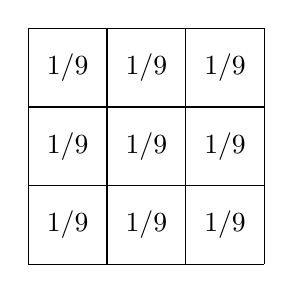
\begin{tikzpicture}
            \draw (0,0) grid (3,3);
            \foreach \u \v in {0.5/0.5,1.5/0.5,2.5/0.5,0.5/1.5,1.5/1.5,2.5/1.5,0.5/2.5,1.5/2.5,2.5/2.5}
            \node at (\u,\v) {\(1/9\)};
        \end{tikzpicture}
        \subcaption{平滑化フィルタ}
        \label{fig:平滑化フィルタ}
    \end{minipage}
    \begin{minipage}[b]{.24\textwidth}
        \centering
        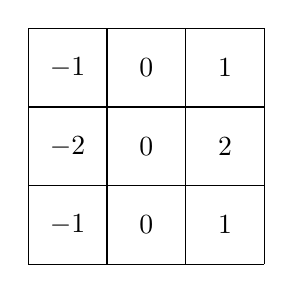
\begin{tikzpicture}
            \draw (0,0) grid (3,3);
            \foreach \u \v \w in {0.5/0.5/{\(-1\)},1.5/0.5/{\(0\)},2.5/0.5/{\(1\)},0.5/1.5/{\(-2\)},1.5/1.5/{\(0\)},2.5/1.5/{\(2\)},0.5/2.5/{\(-1\)},1.5/2.5/{\(0\)},2.5/2.5/{\(1\)}}
            \node at (\u,\v) {\w};
        \end{tikzpicture}
        \subcaption{Prewittフィルタ:横方向}
        \label{fig:Prewittフィルタ_横方向}
    \end{minipage}
    \begin{minipage}[b]{.24\textwidth}
        \centering
        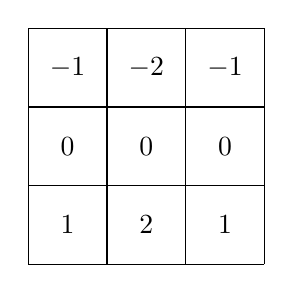
\begin{tikzpicture}
            \draw (0,0) grid (3,3);
            \foreach \u \v \w in {0.5/0.5/{\(1\)},1.5/0.5/{\(2\)},2.5/0.5/{\(1\)},0.5/1.5/{\(0\)},1.5/1.5/{\(0\)},2.5/1.5/{\(0\)},0.5/2.5/{\(-1\)},1.5/2.5/{\(-2\)},2.5/2.5/{\(-1\)}}
            \node at (\u,\v) {\w};
        \end{tikzpicture}
        \subcaption{Prewittフィルタ:縦方向}
        \label{fig:Prewittフィルタ_縦方向}
    \end{minipage}
    \begin{minipage}[b]{.24\textwidth}
        \centering
        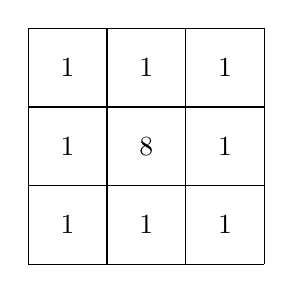
\begin{tikzpicture}
            \draw (0,0) grid (3,3);
            \foreach \u \v in {0.5/0.5,1.5/0.5,2.5/0.5,0.5/1.5,2.5/1.5,0.5/2.5,1.5/2.5,2.5/2.5}
            \node at (\u,\v) {\(1\)};
            \node at (1.5,1.5) {\(8\)};
        \end{tikzpicture}
        \subcaption{ラプラシアンフィルタ}
        \label{fig:ラプラシアンフィルタ}
    \end{minipage}
    \caption{\(3\times 3\)画像フィルタ}
\end{figure}
\paragraph{色空間変換}この実験では,RGB色空間から,HSV色空間へ変換する.RGB色空間は,赤(Red),緑(Green),青(Blue)の3チャネルで構成する.HSVは色相(Hue),彩度(Saturation),明度(Value)の3チャネルで構成する.
色相は,カラー ホイール上の色の位置に対応する,\(0\)から\(100\)の値,色相の量または中間からの逸脱.特定の色の赤,緑,青成分の中での最大値.いずれも\texttt{double}型で保存される\cite{rgb2hsv}.
HSV色空間の特徴として,人間が色を知覚する方法と類似しており,視覚障害者向けのアクセシビリティ向上に役立つことが挙げられる.たとえば,HSVの「明度」を調節することで,文字が見やすくなる\cite[p.97\ -\ p.98]{画像処理}.
また,人間が色を知覚する方法と類似していることを踏まえて,HSV色空間を用いることで,画像の特徴を抽出しやすくなる.
今回の実験では,自分の手の写真をRGB色空間からHSV色空間へ変換し,肌色領域を抽出する.抽出した肌色領域を白色,そのほかの部分を黒色にして出力する.出力した画像と,RGB色空間における肌色領域を抽出した場合の精度について考察する.

\begin{wrapfigure}{r}[0mm]{.3\textwidth}
    \vspace{-.5cm}
    \begin{lstlisting}[caption={白色ガウス雑音画像の生成},label={src:白色ガウス雑音画像の生成}]
% 画像サイズ : n x m
wgn = 10*randn(n, m);
wgn = uint8(wgn);
wgn_img = wgn + gimg;
    \end{lstlisting}
    \begin{lstlisting}[caption={インパルス雑音画像の生成},label={src:インパルス雑音画像の生成}]
% 画像サイズ : n x m
rnd = rand(n, m);
b = (rnd < 0.01);
w = (rnd > 0.99);
in_img(w) = 255;
in_img(b) = 0;
    \end{lstlisting}
    \vspace{-1cm}
\end{wrapfigure}
\section{\method}
\paragraph{白色ガウス雑音を加えた画像}
白色ガウス雑音の作成には\texttt{randn}関数を用い,生成した乱数と,標準偏差の積を取る.生成した乱数を\texttt{uint8}型に変換し,\originimg と和を取る(\srcref{src:白色ガウス雑音画像の生成}).
\(255\)を上回る,または\(0\)を下回る場合,それぞれの値に変換したものを, \wgnimg とする.
\paragraph{インパルス雑音を加えた画像}
インパルス雑音は,\texttt{rand}関数を用いて作成する.発生率を\(1\%\) にするため,乱数の\(0.01\)未満の画素を黒,乱数の\(0.99\)より大きい画素を白としてインパルスノイズを設計する(\srcref{src:インパルス雑音画像の生成}).
\paragraph{フィルタの適用}
平滑化フィルタ,微分フィルタ,ラプラシアンフィルタの適用は,\texttt{filter2}関数,(\ \verb|filter2(filter, img)|\ )を用いる.
メディアンフィルタは,画像の\mat{i}{j}に対して,\texttt{median}関数を用いてフィルタ処理する.メディアンフィルタを適用する際に,四方に画素がない画素(\mat{1}{1}画素,\mat{m}{1}画素など)はフィルタ処理できないため,0パディング処理を行い,メディアンフィルタを適用する(\srcref{src:メディアンフィルタの適用}).
\begin{lstlisting}[caption={メディアンフィルタの適用},label={src:メディアンフィルタの適用},frame={left}]
for h = 2:img_height % 画像行列 img の高さ
    for w = 2:img_width % 画像行列 img の横幅,median_filter は0パディング後のimg
        median_filter(h-1, w-1) = median(img(h-1:h+1,w-1:w+1),"all"); 
    end
end
\end{lstlisting}
課題(フィルタ処理)のスクリプトは,\sref{src:06_01} - \sref{src:06_04}.
\paragraph{色空間変換}
読み込んだ画像はRGB色空間で保存される.この画像をHSV色空間に変換するためには,\texttt{rgb2hsv}関数を用いる.
出力された値と\(255\)の積を取り,HSV色空間で出力された画像を書き出す.
色相,彩度,明度それぞれのチャネルを抽出し,\matlab のアプリケーションを用いて,肌色要素のHSV成分を出力する(\sref{src:06_05_f}).
それぞれの値に合致した画素を,画素値\(255\),ほかの画素値を\(0\)とした画像を書き出す.また,RGB色空間における,肌色領域の抽出も行う.肌色部ある点のRGB値と等しい画素を白く塗る.
\scall{\kadaibe}\sref{src:06_05},\sref{src:06_05_1}.
\section{\result}
\begin{figure}[h]
    \centering
    \begin{minipage}[b]{.3\textwidth}
        \centering
        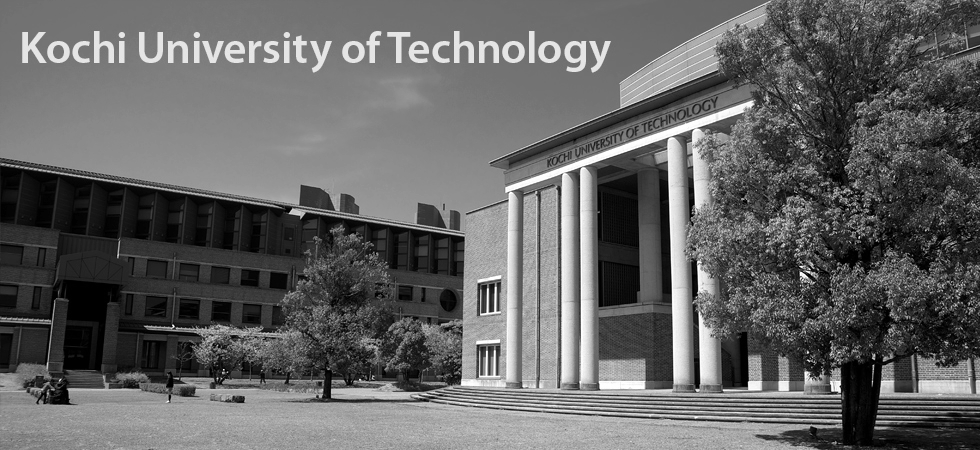
\includegraphics[keepaspectratio,width=\textwidth]{../../Figures/05_21_gimg.png}
        \subcaption{元画像}
    \end{minipage}
    \begin{minipage}[b]{.3\textwidth}
        \centering
        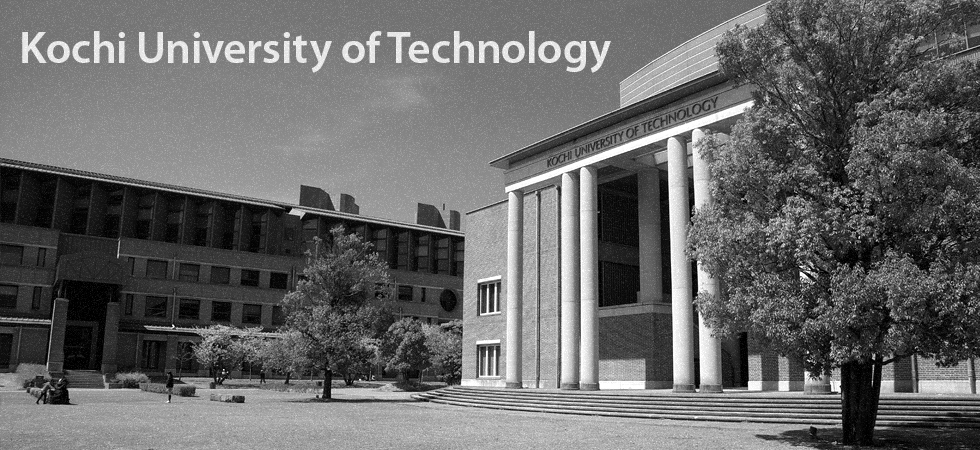
\includegraphics[keepaspectratio,width=\textwidth]{../../06_ImageFiltering/file_white-Gaussian-Noise.png}
        \subcaption{白色ガウス雑音(\wgnimg)}
    \end{minipage}
    \begin{minipage}[b]{.3\textwidth}
        \centering
        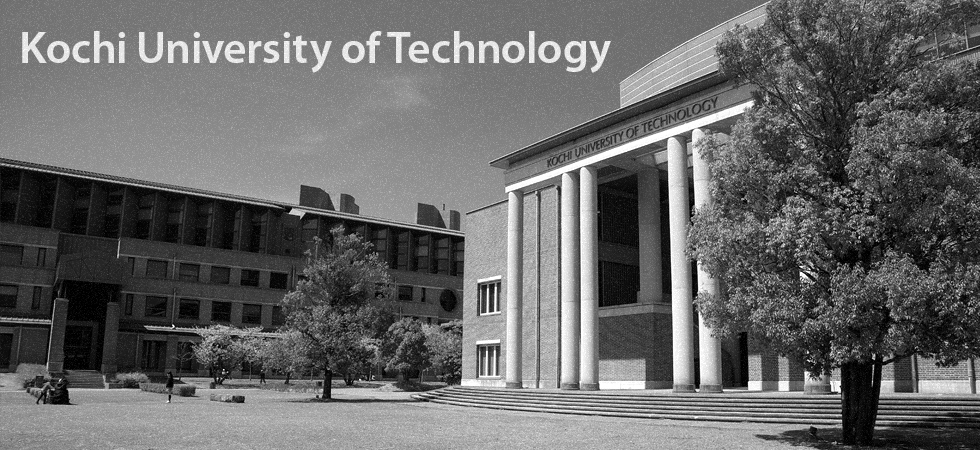
\includegraphics[keepaspectratio,width=\textwidth]{../../06_ImageFiltering/file_impluse-noise.png}
        \subcaption{インパルス雑音(\inimg)}
    \end{minipage}
    \caption{\kadaiaa\ 実験結果}
    \begin{minipage}[b]{.49\textwidth}
        \begin{minipage}[b]{.49\textwidth}
            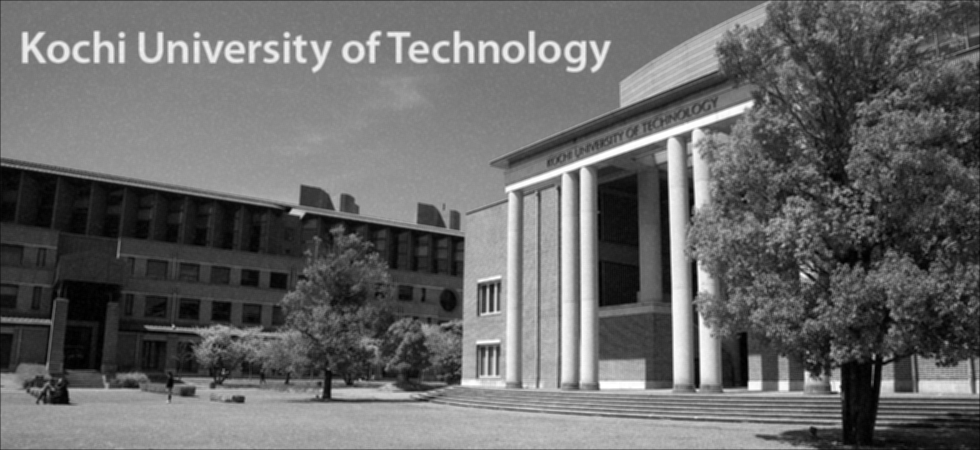
\includegraphics[keepaspectratio,width=\textwidth]{../../Figures/06_21_sf_img_wgn.png}
            \subcaption{\wgnimg}
        \end{minipage}
        \begin{minipage}[b]{.49\textwidth}
            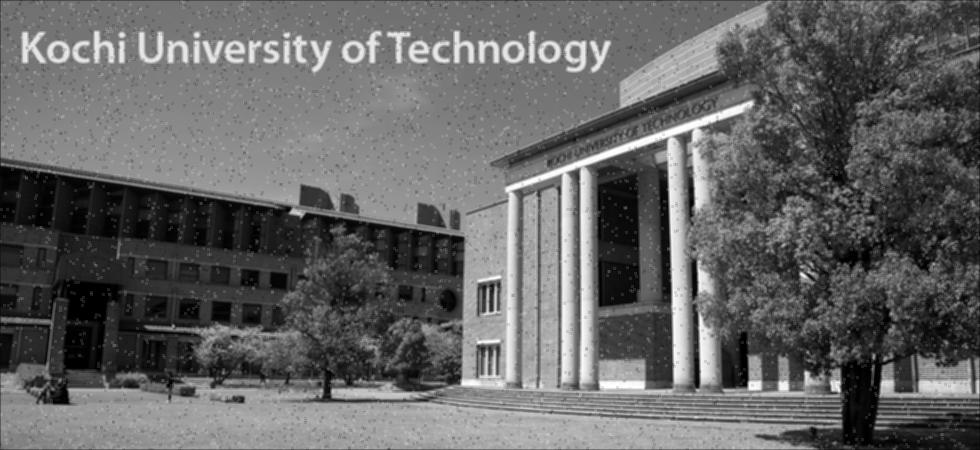
\includegraphics[keepaspectratio,width=\textwidth]{../../Figures/06_22_sf_img_in.png}
            \subcaption{\inimg}
        \end{minipage}
        \caption{平滑化フィルタ}
    \end{minipage}
    \begin{minipage}[b]{.49\textwidth}
        \begin{minipage}[b]{.49\textwidth}
            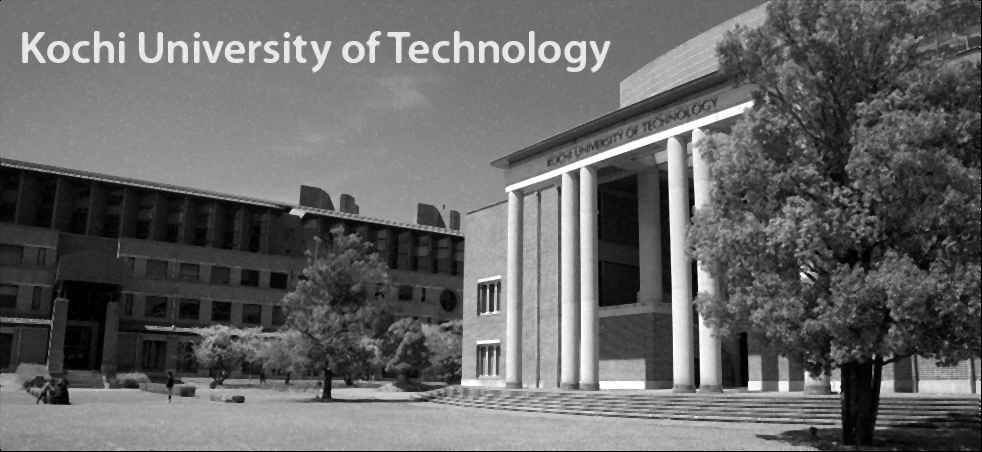
\includegraphics[keepaspectratio,width=\textwidth]{../../Figures/06_23_mf_img_wgn.png}
            \subcaption{\wgnimg}
        \end{minipage}
        \begin{minipage}[b]{.49\textwidth}
            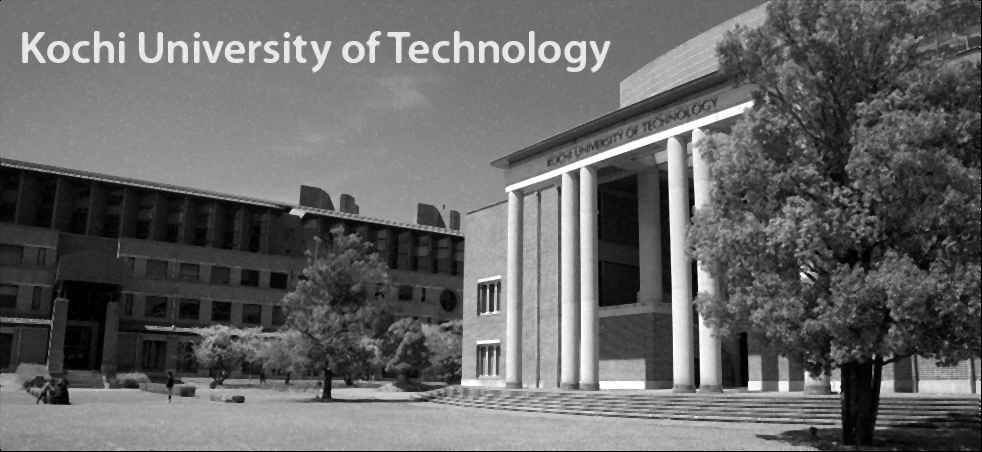
\includegraphics[keepaspectratio,width=\textwidth]{../../Figures/06_24_mf_img_in.png}
            \subcaption{\inimg}
        \end{minipage}
        \caption{メディアンフィルタ}
    \end{minipage}
    \begin{minipage}[b]{.3\textwidth}
        \centering
        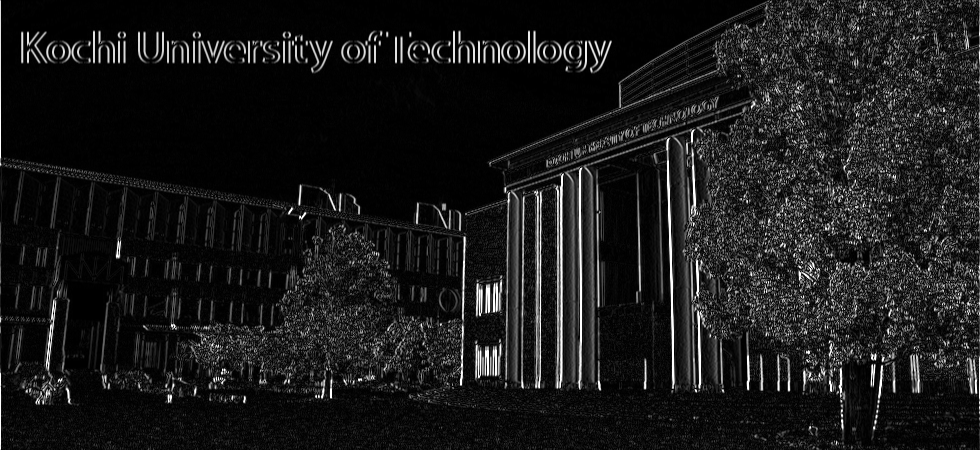
\includegraphics[keepaspectratio,width=\textwidth]{../../Figures/06_31_diff-x-img.png}
        \subcaption{横方向微分フィルタ}
    \end{minipage}
    \begin{minipage}[b]{.3\textwidth}
        \centering
        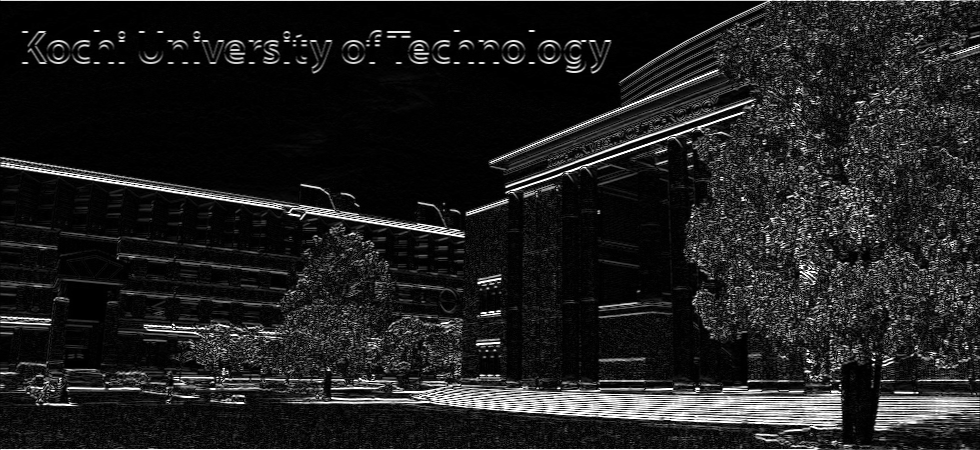
\includegraphics[keepaspectratio,width=\textwidth]{../../Figures/06_32_diff-y-img.png}
        \subcaption{縦方向微分フィルタ}
    \end{minipage}
    \begin{minipage}[b]{.3\textwidth}
        \centering
        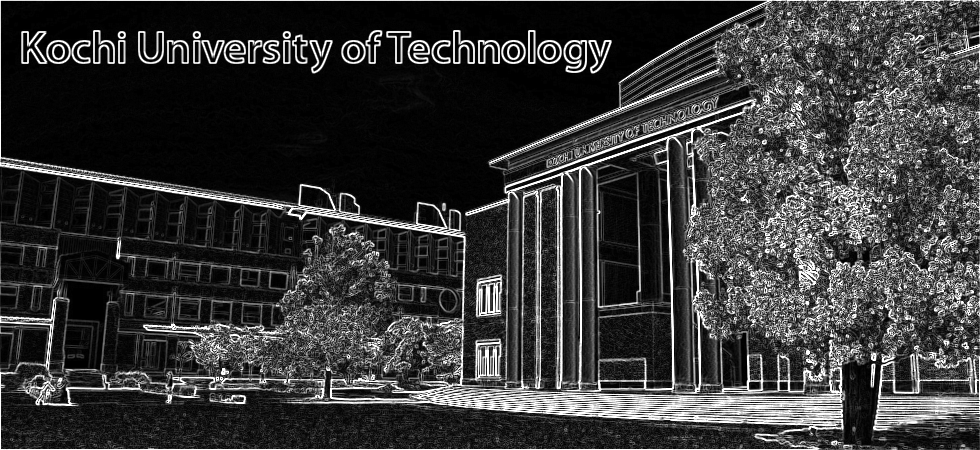
\includegraphics[keepaspectratio,width=\textwidth]{../../Figures/06_33_diff-img.png}
        \subcaption{微分フィルタ\footnotemark}
    \end{minipage}
    \caption{微分フィルタ適用}
    \begin{minipage}[b]{.3\textwidth}
        \centering
        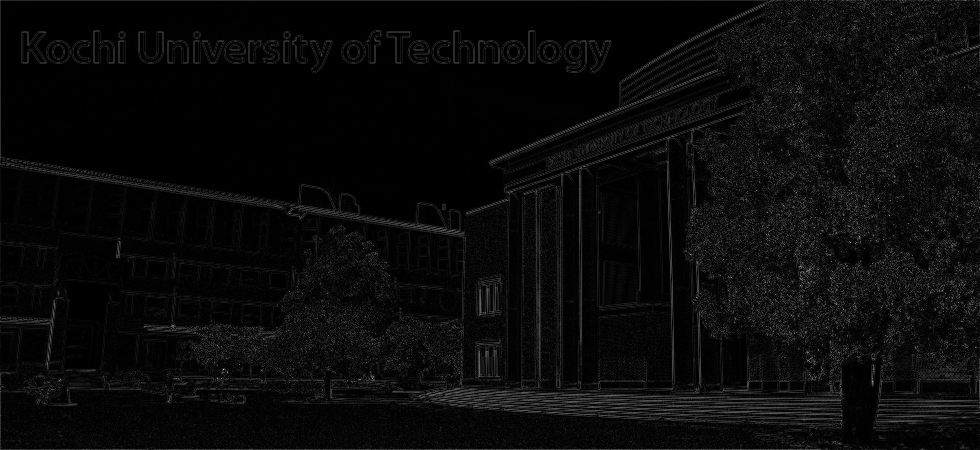
\includegraphics[keepaspectratio,width=\textwidth]{../../Figures/06_41_lf-img}
        \subcaption{ラプラシアンフィルタ}
    \end{minipage}
    \begin{minipage}[b]{.3\textwidth}
        \centering
        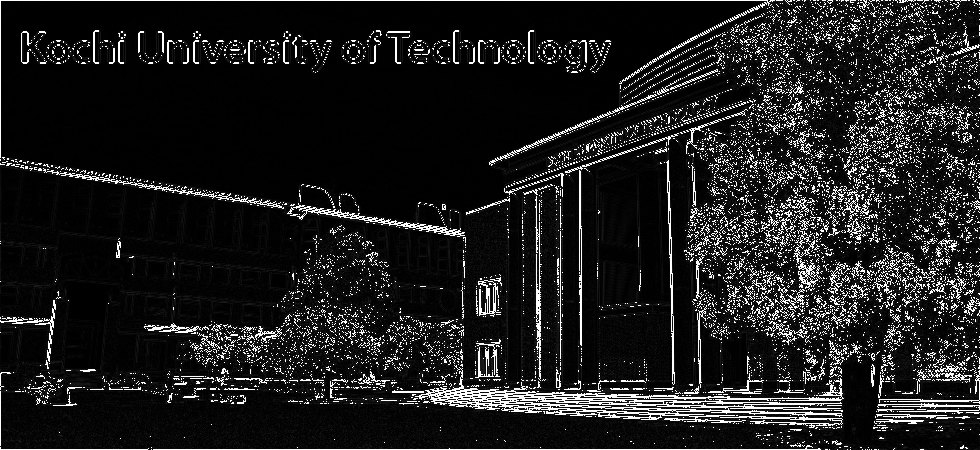
\includegraphics[keepaspectratio,width=\textwidth]{../../Figures/06_43_lf-img-thresholding.png}
        \subcaption{閾値処理}
    \end{minipage}
    \begin{minipage}[b]{.3\textwidth}
        \centering
        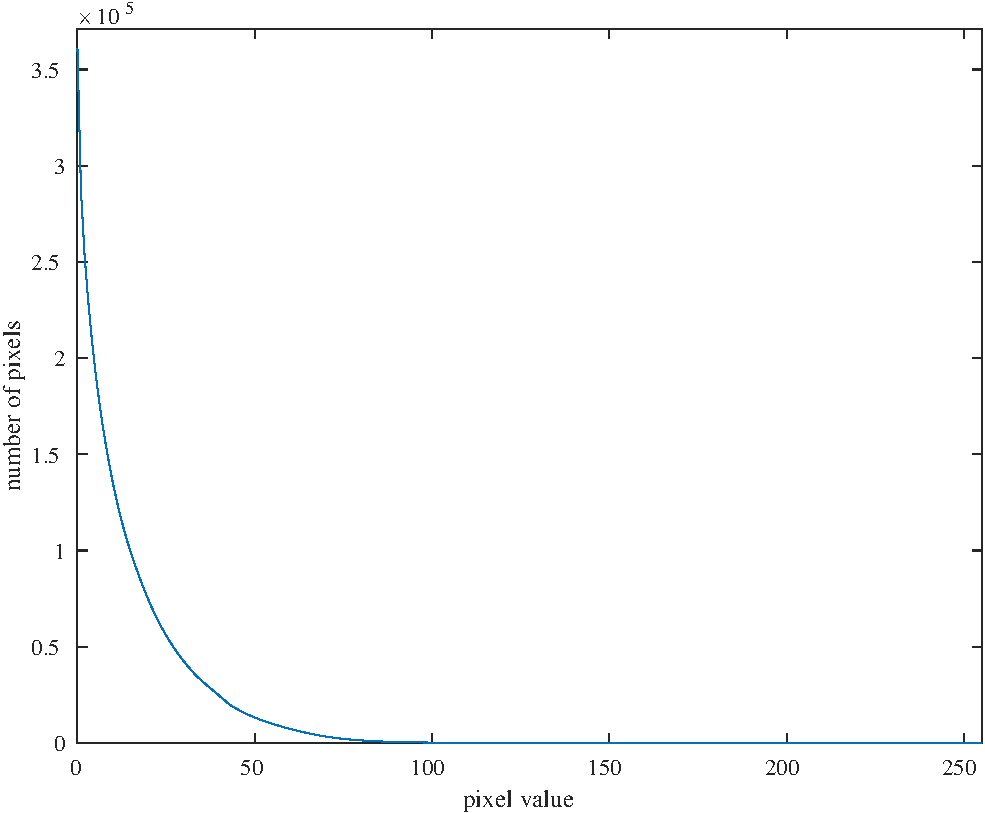
\includegraphics[keepaspectratio,width=\textwidth]{../../Figures/06_42_Thresholding-graph.pdf}
        \subcaption{画素値ヒストグラム}
    \end{minipage}
    \caption{ラプラシアンフィルタの適用と処理}
\end{figure}
\footnotetext{横方向微分フィルタ適用後画像と縦方向微分フィルタ適用後画像の和.}
\begin{figure}[ht]
    \centering
    \begin{minipage}[b]{.23\textwidth}
        \centering
        \includegraphics[keepaspectratio,width=\textwidth]{../../06_ImageFiltering/file_hand.png}
        \subcaption{元画像}
    \end{minipage}
    \begin{minipage}[b]{.23\textwidth}
        \centering
        \includegraphics[keepaspectratio,width=\textwidth]{../../Figures/06_51_img-hsv.png}
        \subcaption{HSV色空間への変換後}
    \end{minipage}
    \begin{minipage}[b]{.23\textwidth}
        \centering
        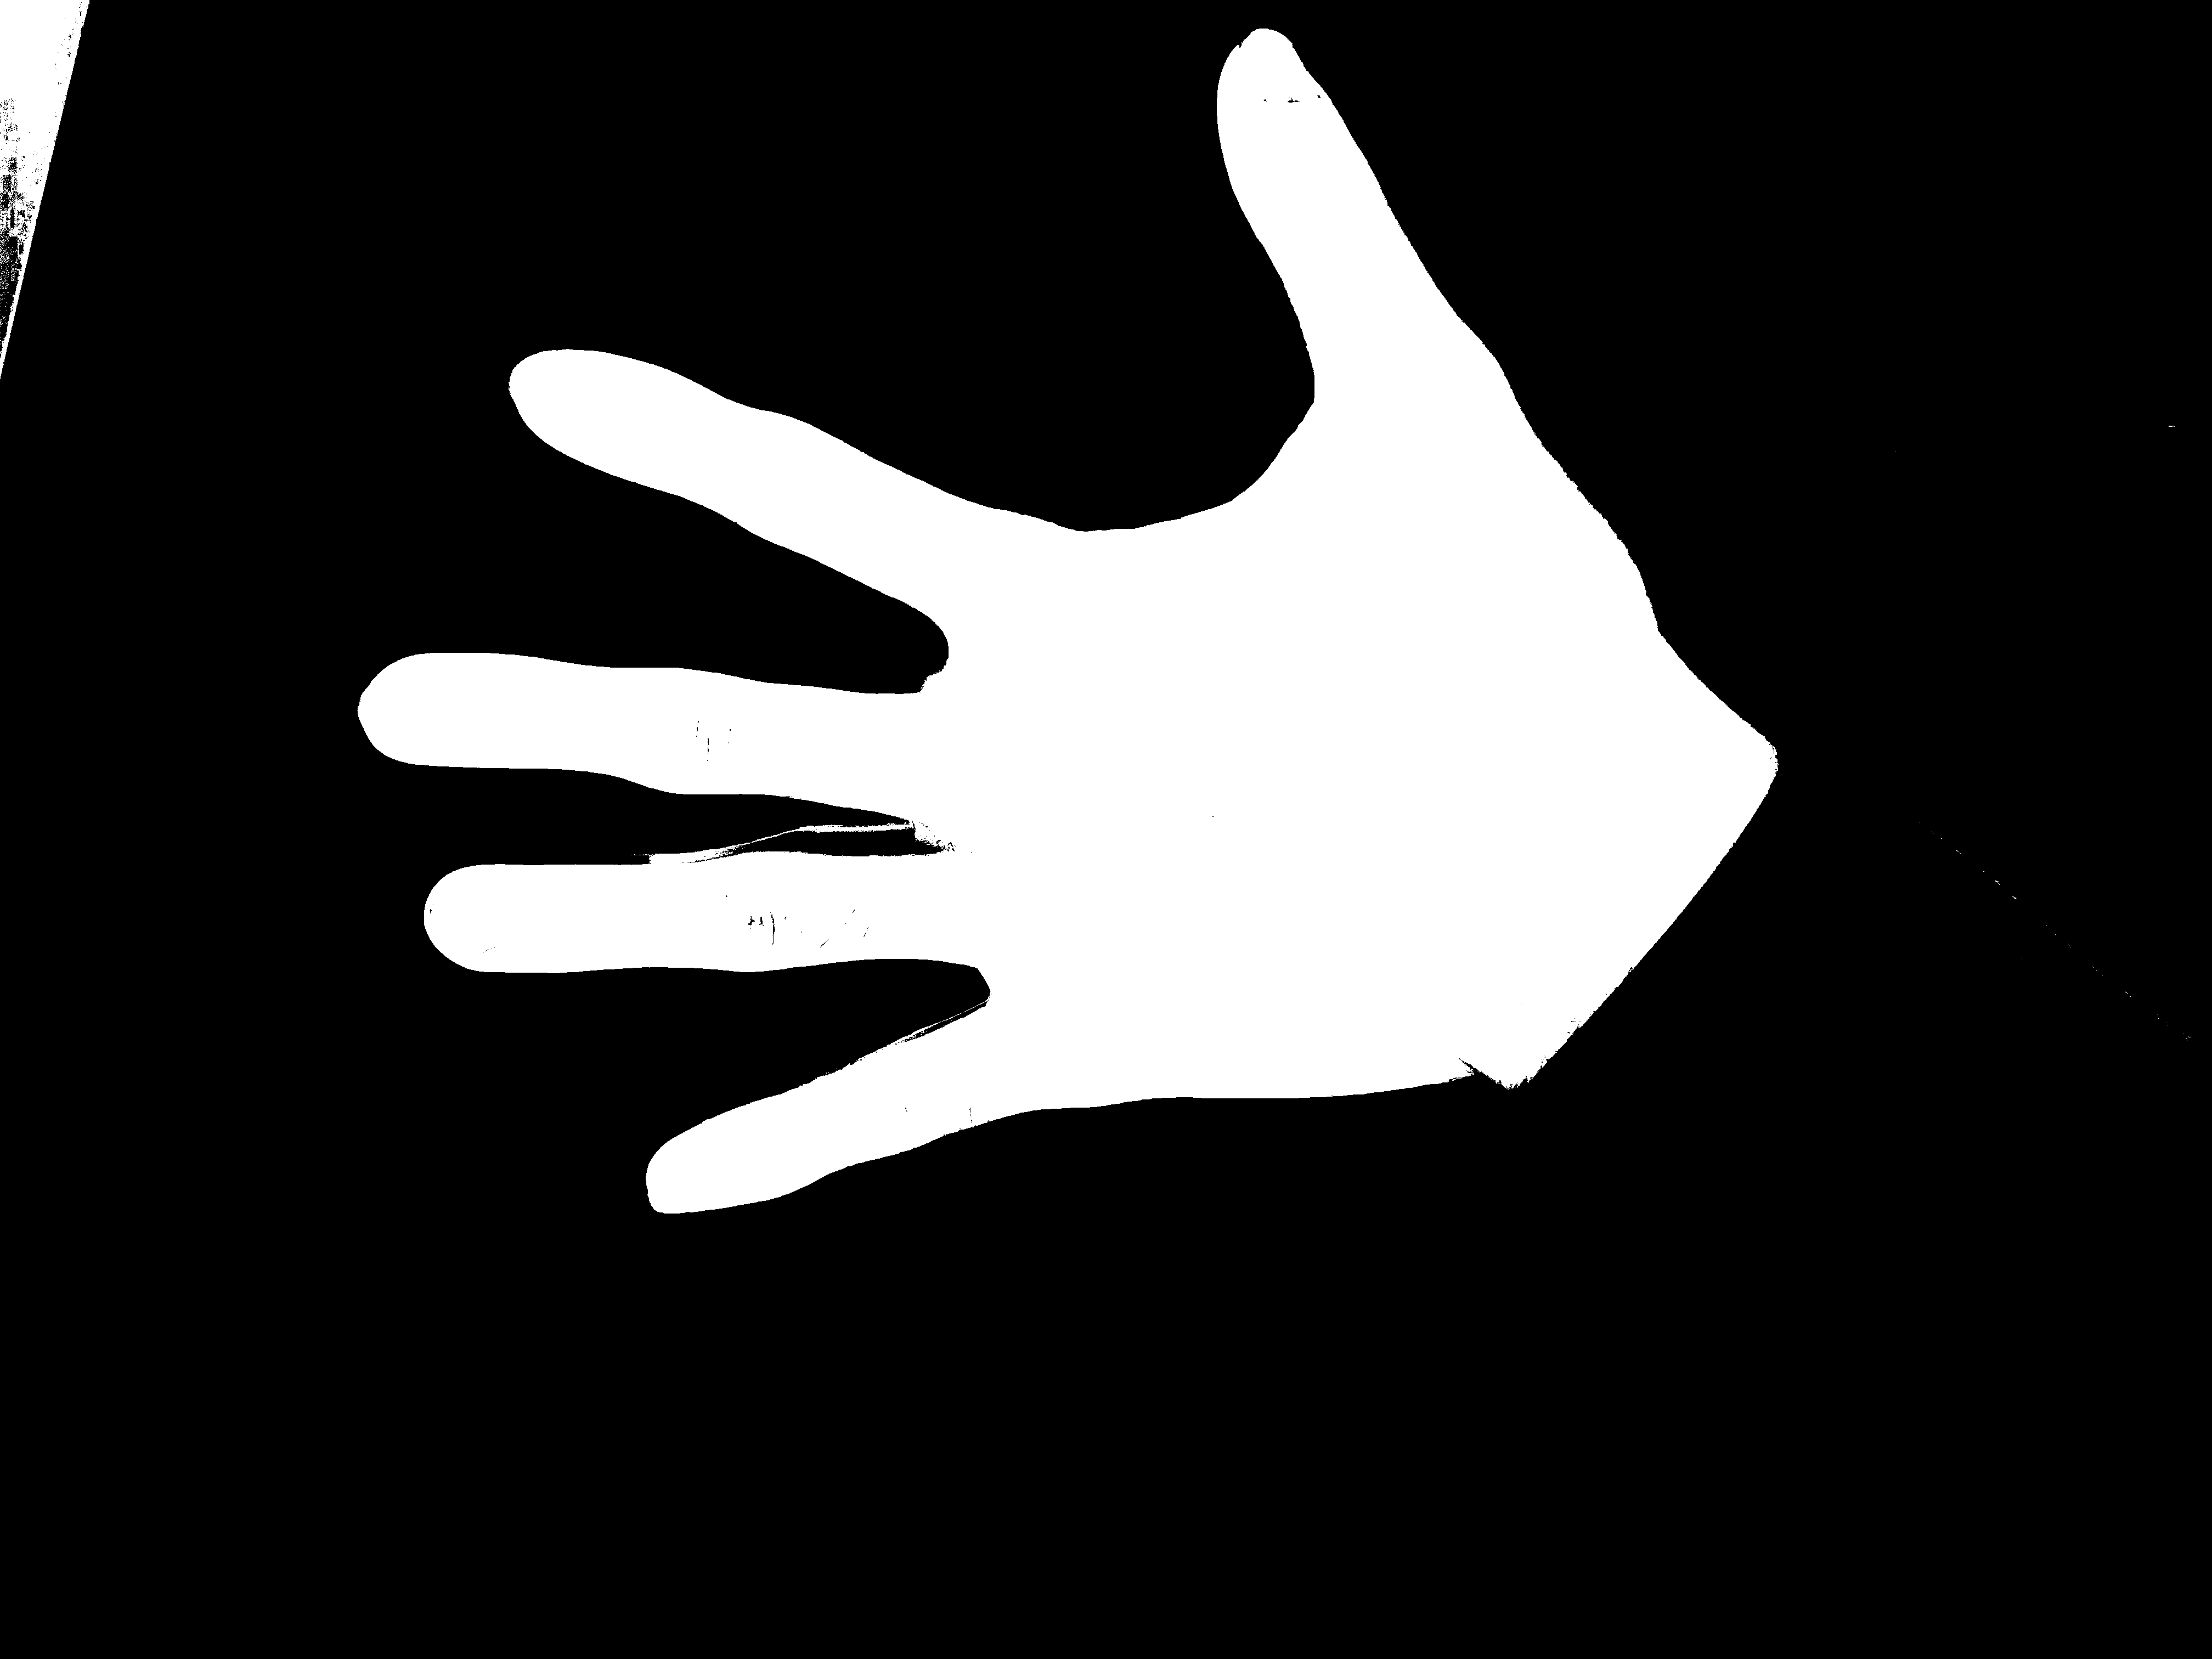
\includegraphics[keepaspectratio,width=\textwidth]{../../Figures/06_52_scd.png}
        \subcaption{肌色領域の抽出(HSV)}
    \end{minipage}
    \begin{minipage}[b]{.23\textwidth}
        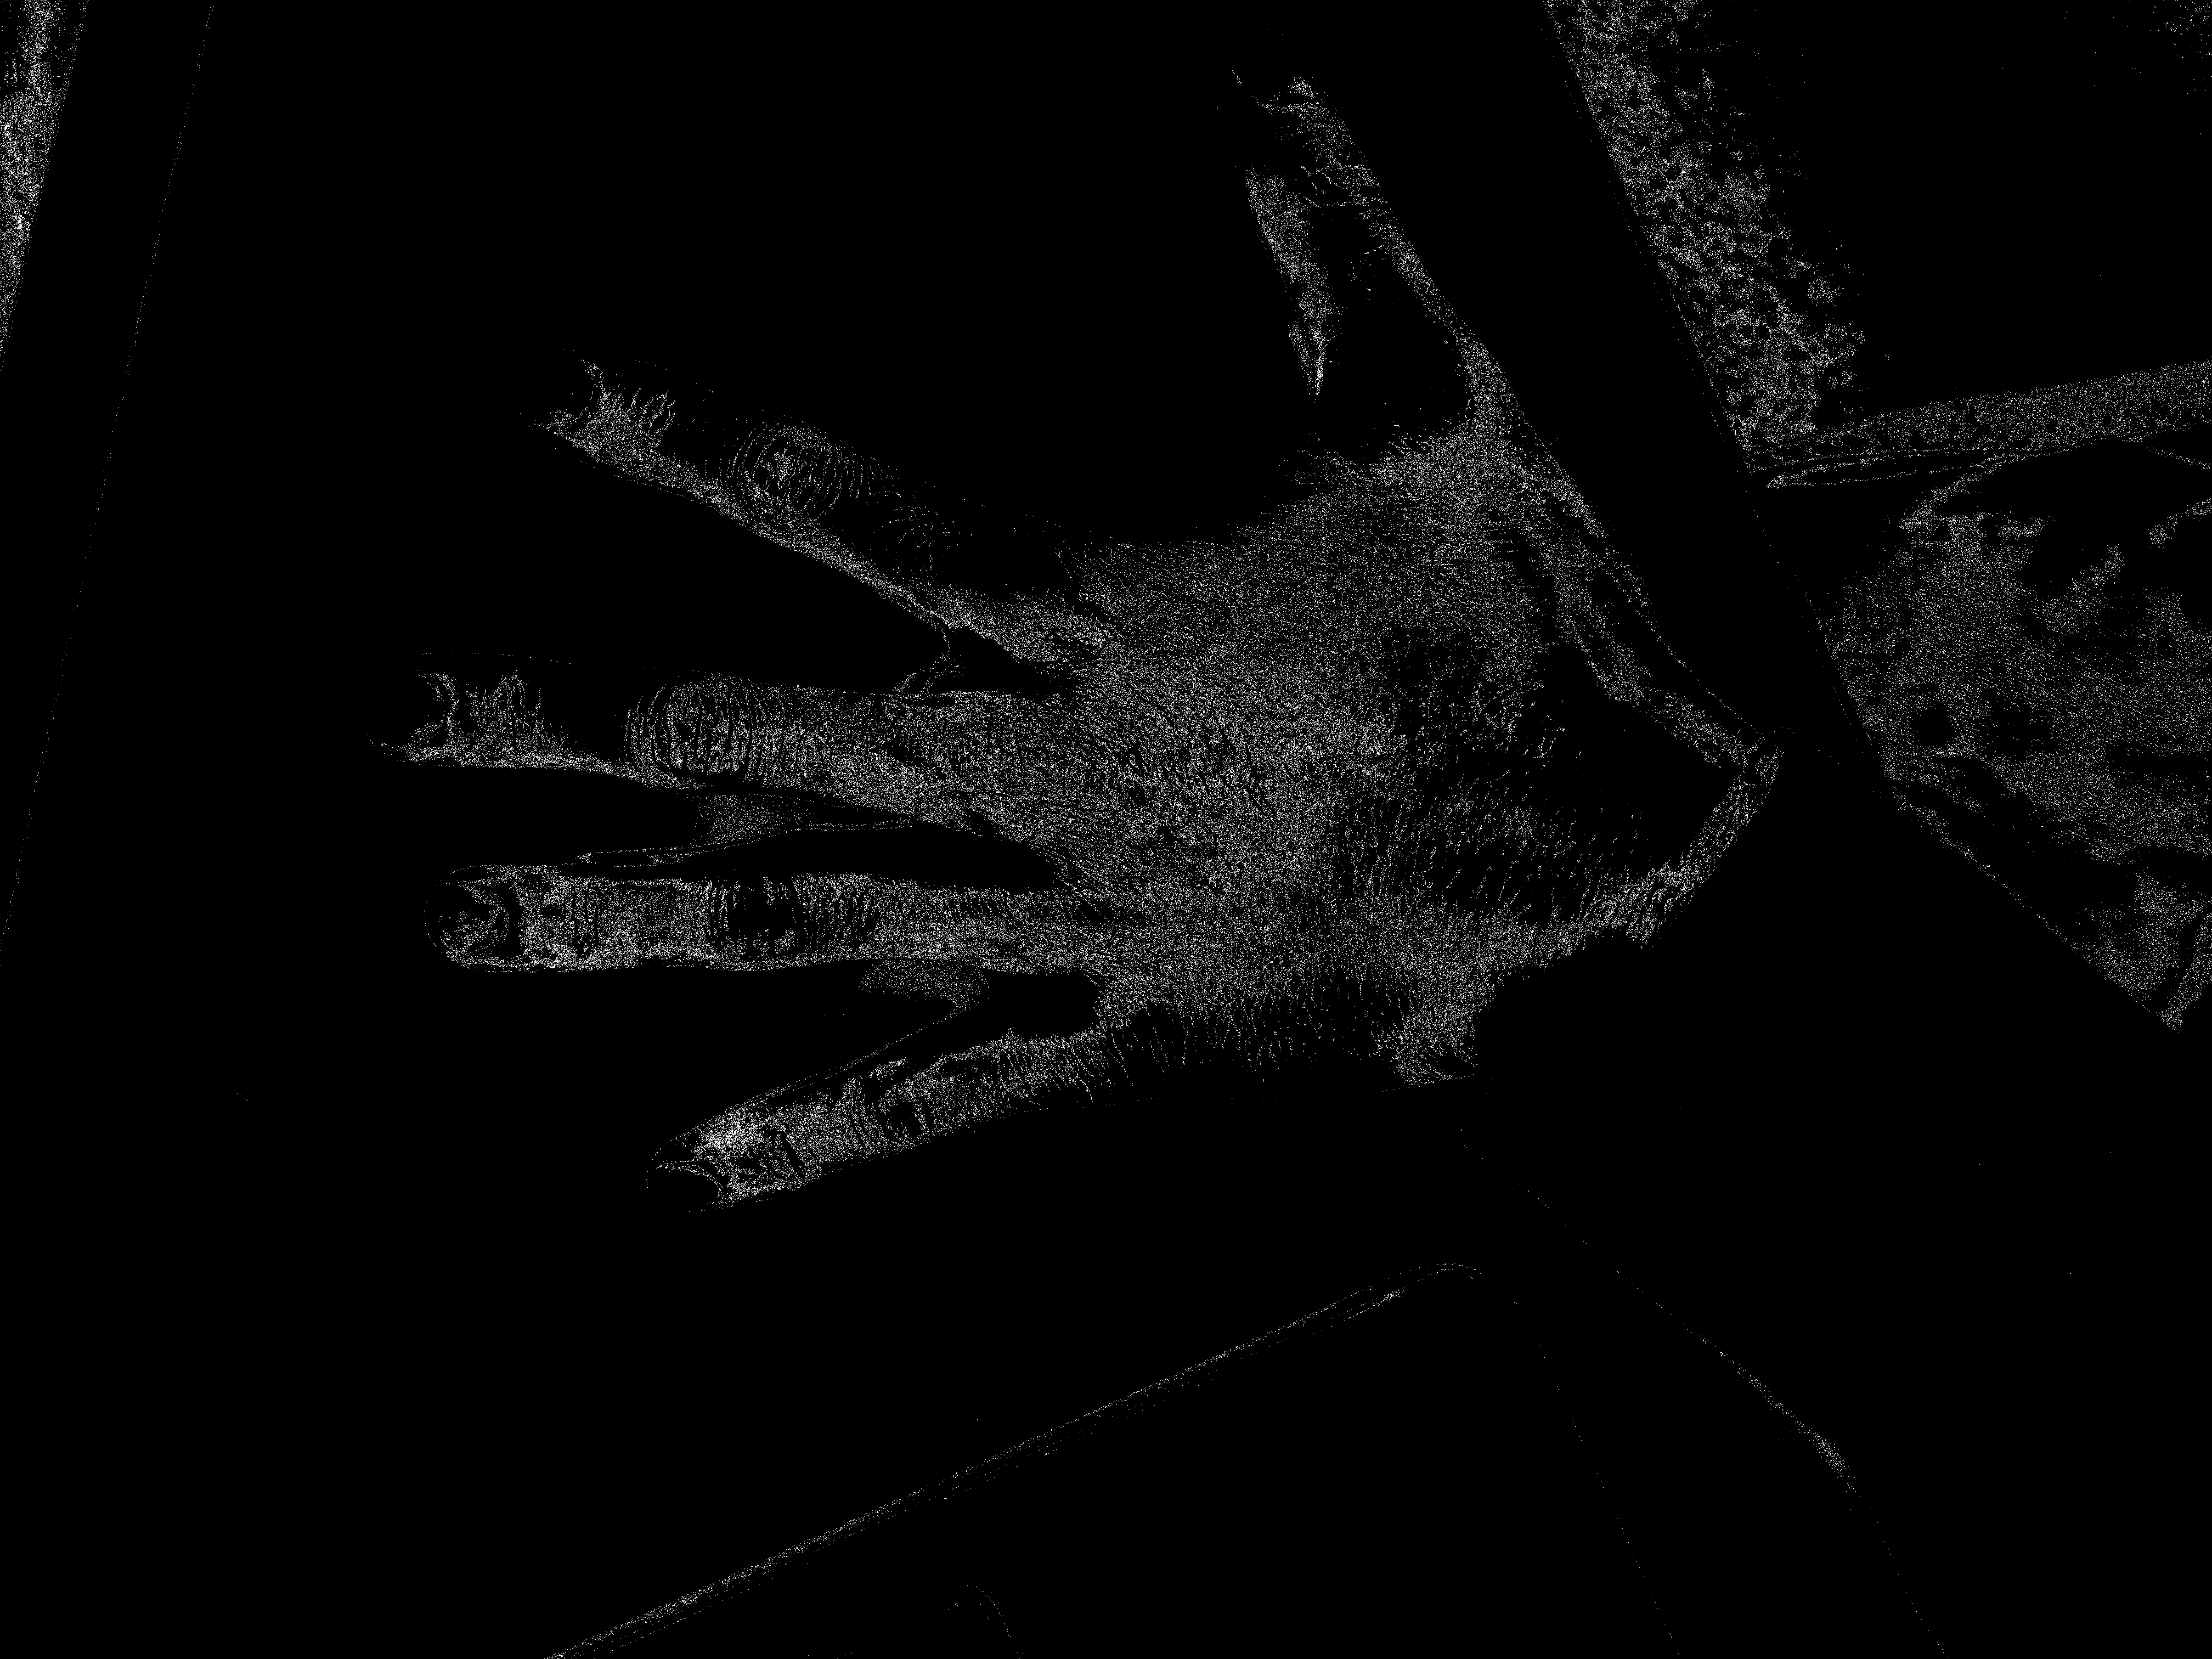
\includegraphics[keepaspectratio,width=\textwidth]{../../Figures/06_53_hand.png}
        \subcaption{肌色領域の抽出(RGB)}
    \end{minipage}
    \caption{\kadaibe\ 実験結果}
\end{figure}
\section{\consideration}
\paragraph{平滑化フィルタ,メディアンフィルタ}
\wgnimg に対して平滑化フィルタを適用すると,雑音部分が目立たなくなった.また,\inimg に対して平滑化フィルタを適用すると,雑音が取り除かれることなく残った.
\wgnimg と\inimg に対してメディアンフィルタを適用すると,雑音部分が目立たなくなった.